\documentclass[12pt]{article}
\usepackage[a4paper, total={6.5in, 9in}]{geometry}
\parindent = 0pt
\usepackage{amssymb, amsmath}
\usepackage{graphicx}
\usepackage{fancyhdr}
\usepackage{listings}
\lstdefinestyle{chstyle}{
basicstyle=\ttfamily\small,
showstringspaces=false,
%captionpos=b,
}
\begin{document}

\pagestyle{fancy}
\fancyhead[L]{0801CS211018}
\fancyhead[R]{Ansh Jain}
\fancyfoot{}
\fancyfoot[R]{\thepage}

\begin{center}
\LARGE{\textbf{MINI PROJECT}}
\end{center}

%objectives
\section{Objective}
The objective of this project is to provide a interface where a hotels can expand their business, people can order food easily, delivery man can work efficiently with the help of this single software. This project helps people to efficiently order food within simple and minimal steps. The project provide an interface to customer and the hotels to interact in a productive manner and result in user friendly outcomes by improving the services regularly.

%function desciption
\section{Function Description}
\subsection{random\_number\_generator}
This function is used to generate random numbers which are used further. Other functions having purpose of login call this function to assign registration ID to the user. This function takes upper limit as a parameter to generate numbers within a certain limit and get desired result.
\subsection{delay}
This function is used to produce a delay of output during runtime of the program. This function uses the standard time.h library of c and runs a empty loop until the desired time duration is reached. The amount of time the function needs to delay is taken as a parameter in the function and used accordingly by other functions when they call it. 
\subsection{hotel\_login}
This function sets up the user to use the services of hotel in the program. This function takes the necessary information from the user about their hotel and store them in the user defined structure of hotel. This function also call the random number generator function to assign the registration ID to the hotel.
\subsection{display\_hotel}
This function displays the entered information by the hotel manager about their hotel and their unique ID. This function also confirms the user that their registration is successful and they can further proceed with other services.
\subsection{hotel\_food}
This function is used to let the hotel manager make their menu and provide their customer with the food they are offering. This function also lets the hotel to set price of their food.
\subsection{display\_menu}
This function is used while the customer is ordering food to show him the menu. It assigns a code to each food and lets the user order their food by selecting the specific code of the respective food item.
\subsection{customer\_login}
This function is another side of the project that is the customer side and it is used to register the customer with the services.
It asks for necessary information like name, address and date of birth. This function also calls random number generator function to assign registration ID to the user.
\subsection{display\_customer}
This function displays the entered information by the customer and their unique ID. This function also confirms the customer that their registration is successful and they can further proceed with other services like ordering food.
\subsection{order}
This function lets the customer create his order. Firstly the display  menu function is called so that the user can decide what he needs to order and then the order is generated and the bill is shown to the user.
\subsection{delivery\_man\_login}
This is yet another section of the service where delivery man can register itself and provide delivery services. This function asks the delivery man to enter necessary information like name, vehicle number etc.
\subsection{display\_delivery\_info}
This function is used once the customer has orders his food and the food is on its way. This function also shows the delivery man information who is handling the order. This function calls the delay function and delays the runtime for 4 seconds to make the program more realistic and show that the the order is being processed.
\subsection{ask\_feedback}
This function asks the customer for his feedback once the order is delivered. This covers the last aspect of the project that is the management side of the services. The feedback is used to improve the services. This function also calls the delay function to reflect the delivery time of the order and hence make the project more realistic.

%profiler report
\section{Profiler Report}
Profiler report provides the dynamic analysis of the program. It is useful for program optimisation and increase performance as it contains various aspects of program like space or time complexity of the program frequency and duration of function calls etc.\\
\subsection{Flat Profile}
The flat profile the amount of time program spent executing each function.\\
\\
This section shows the flat profile report which was obtained using gprof profiler.\\
\\
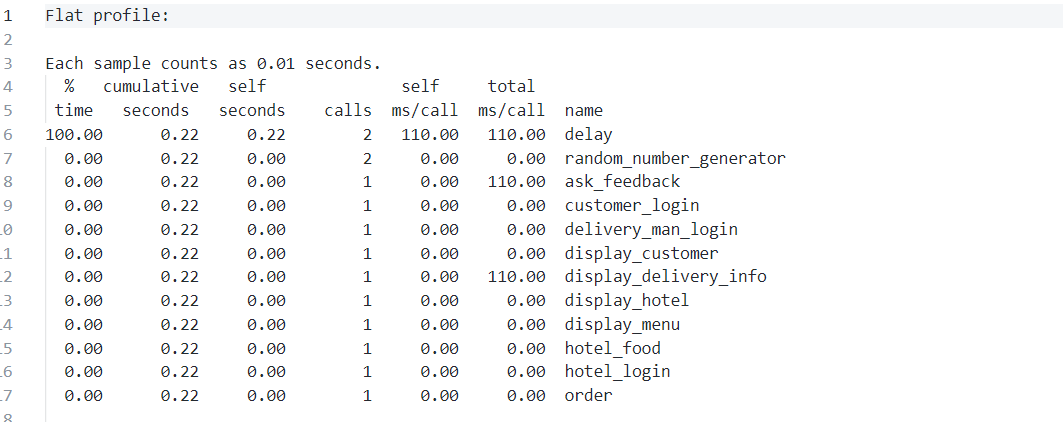
\includegraphics{profile_1.png}\\
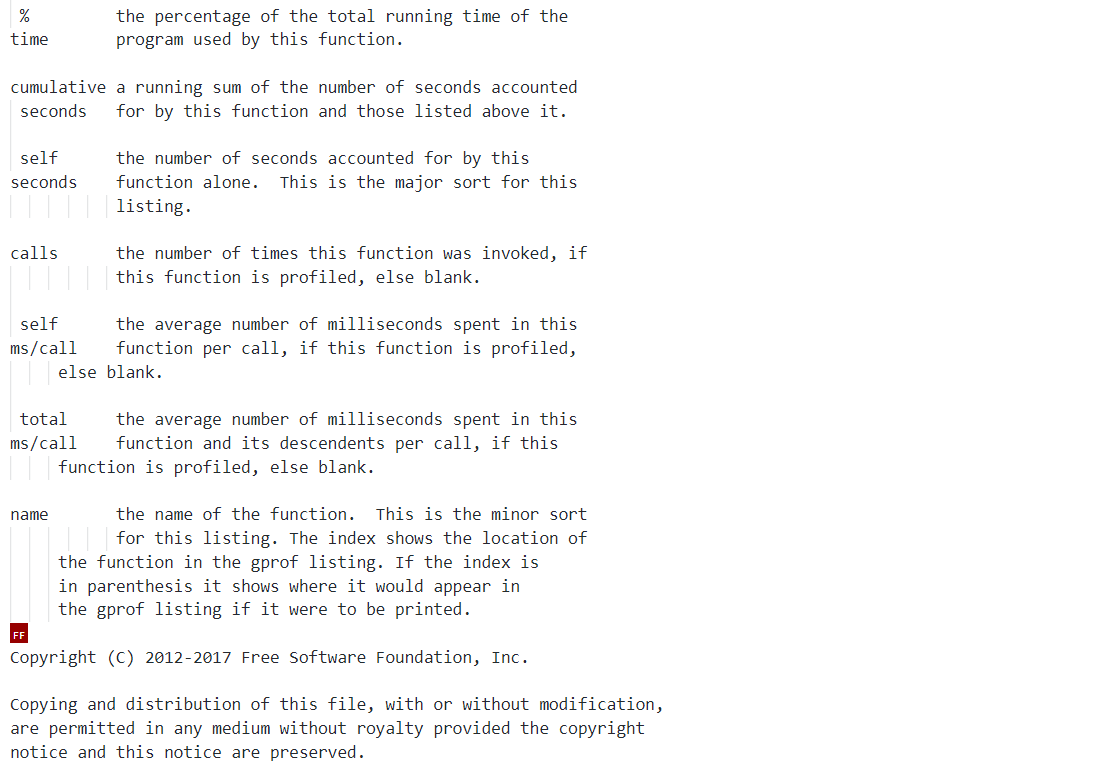
\includegraphics{profile_2.png}\\
\subsection{Call Graph}
The call graph shows the call tree of the program. It shows which function are called by respective function and the other functions that calls the respective function.\\
\\
The functions present above the indexed function(the function which is being analysed) in a section of the call graph are the functions that called the indexed function and the functions present below it are the functions called by the indexed function. \\
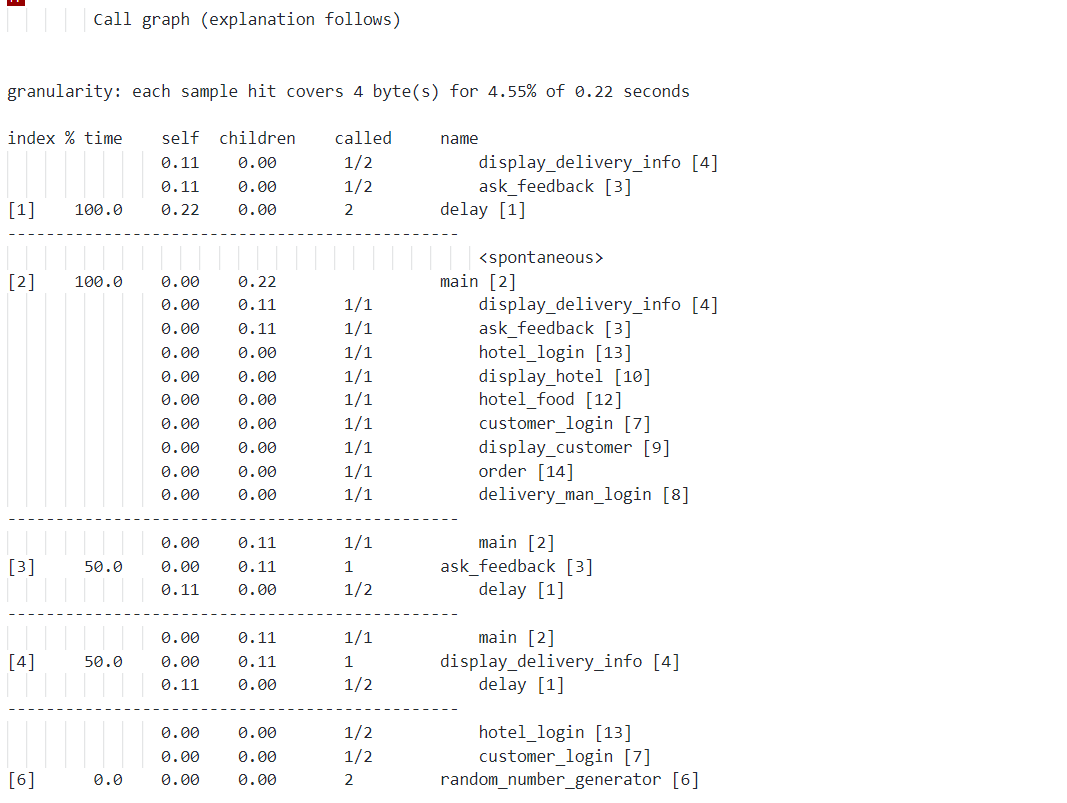
\includegraphics{profile_3.png}\\
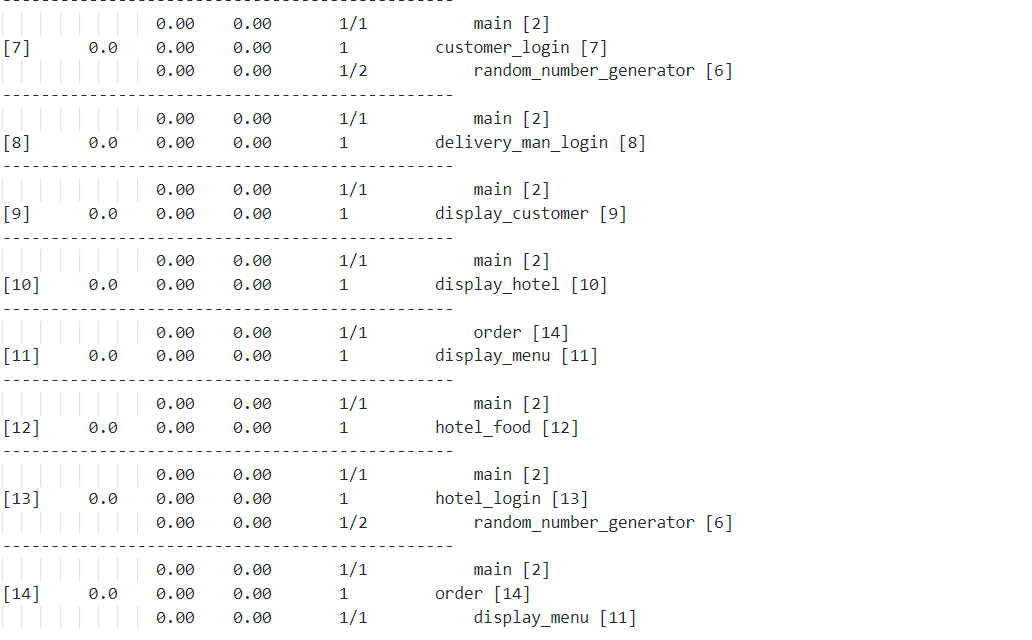
\includegraphics{profile_4.png}\\
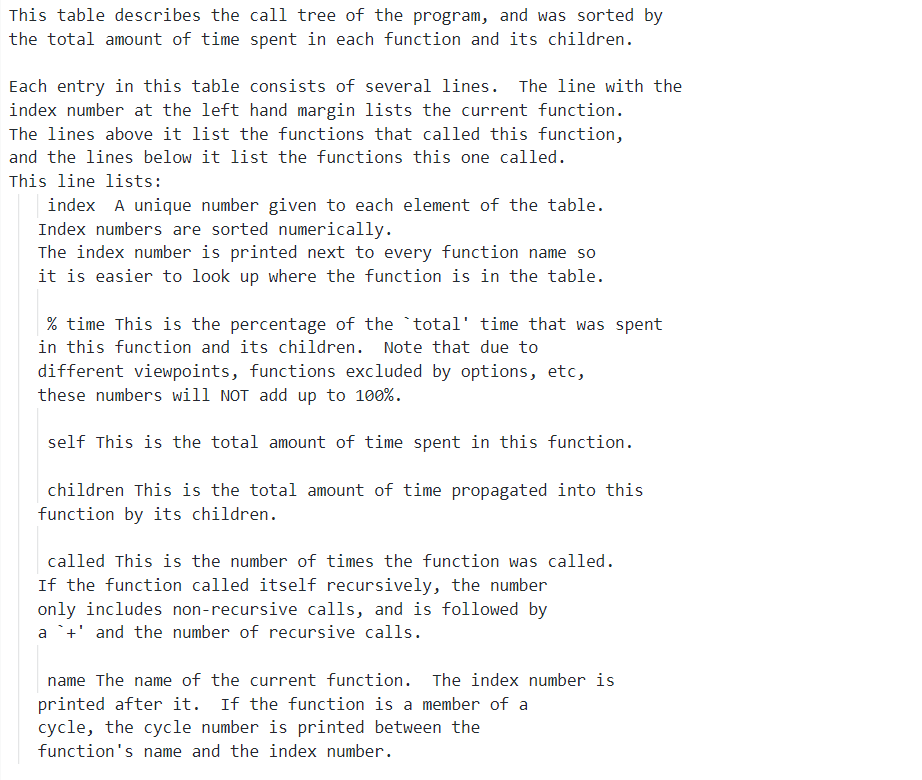
\includegraphics{profile_5.png}\\
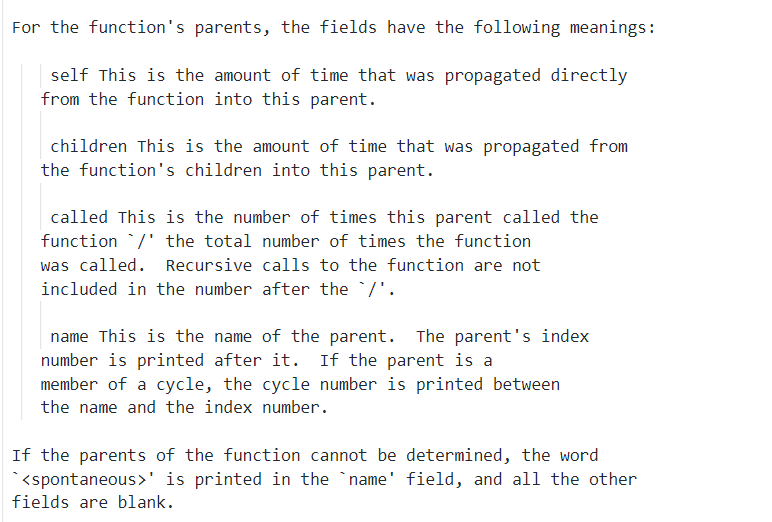
\includegraphics{profile_6.png}\\
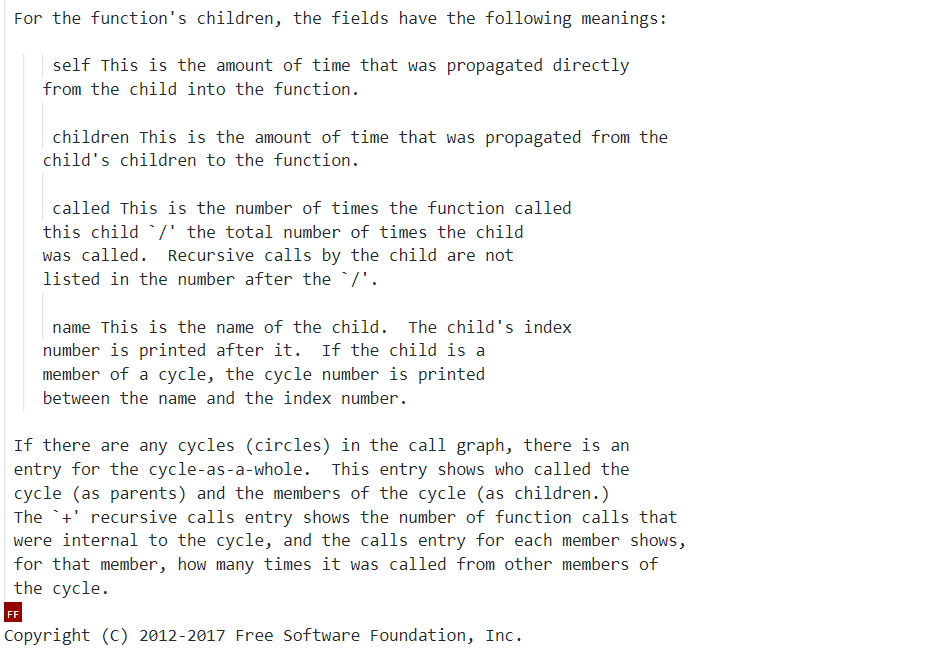
\includegraphics{profile_7.png}\\
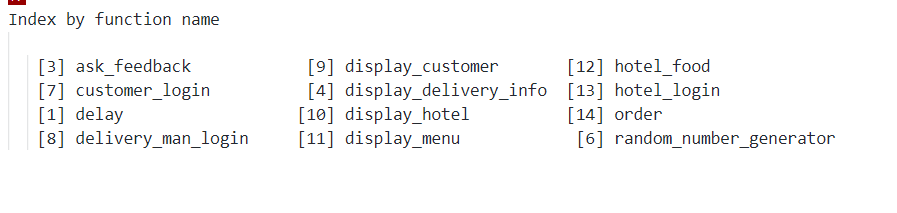
\includegraphics{profile_8.png}\\

%gdb activities
\section{Debugging Process}
Debugging is an important aspect in project development as it is very useful process to identify errors and make the program work as we would like it.\\
\\
\\
The problem in the project was that while the customer was ordering food the first time he the command to read the respective food code didn't work normally.\\
\\
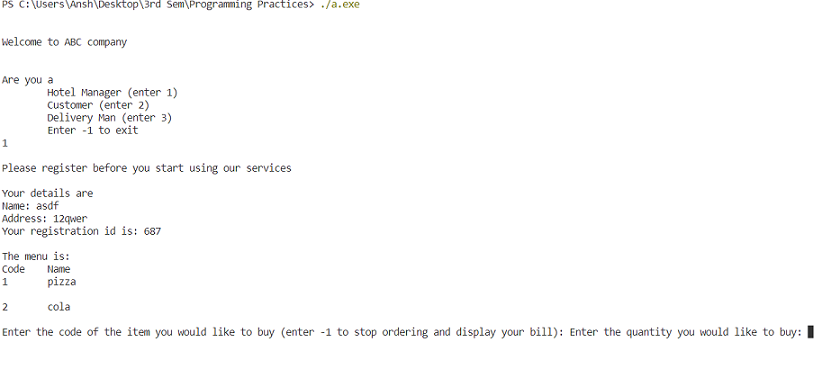
\includegraphics{problem.png} 
\\
As you can see that the program didn't ask for input for the food code.\\
\\
After performing following debugging steps it was identified that the input buffer had \\n in it which was preventing input to be taken, so to solve it a getchar was needed to be introduced, so that it could first remove the \\n from input buffer and then the program would run normally.\\
\\
These are the gdb steps\\
\\
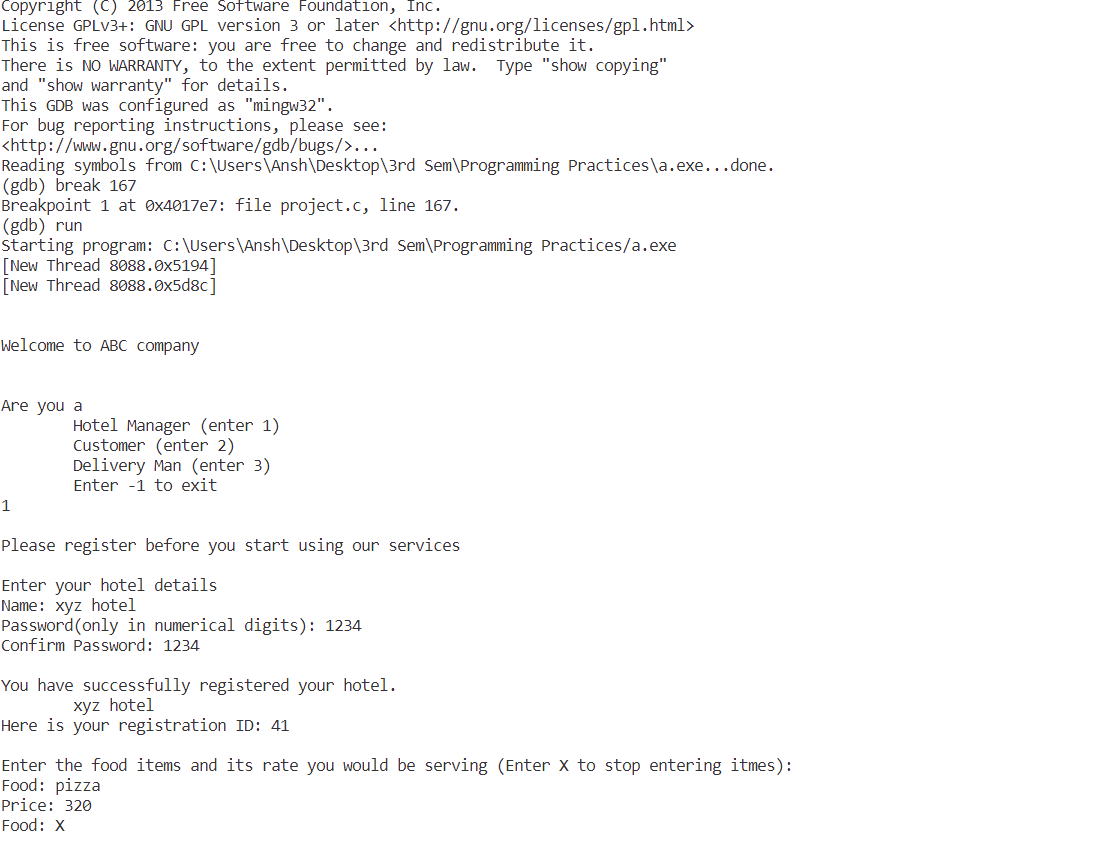
\includegraphics{gdb_1.png}\\
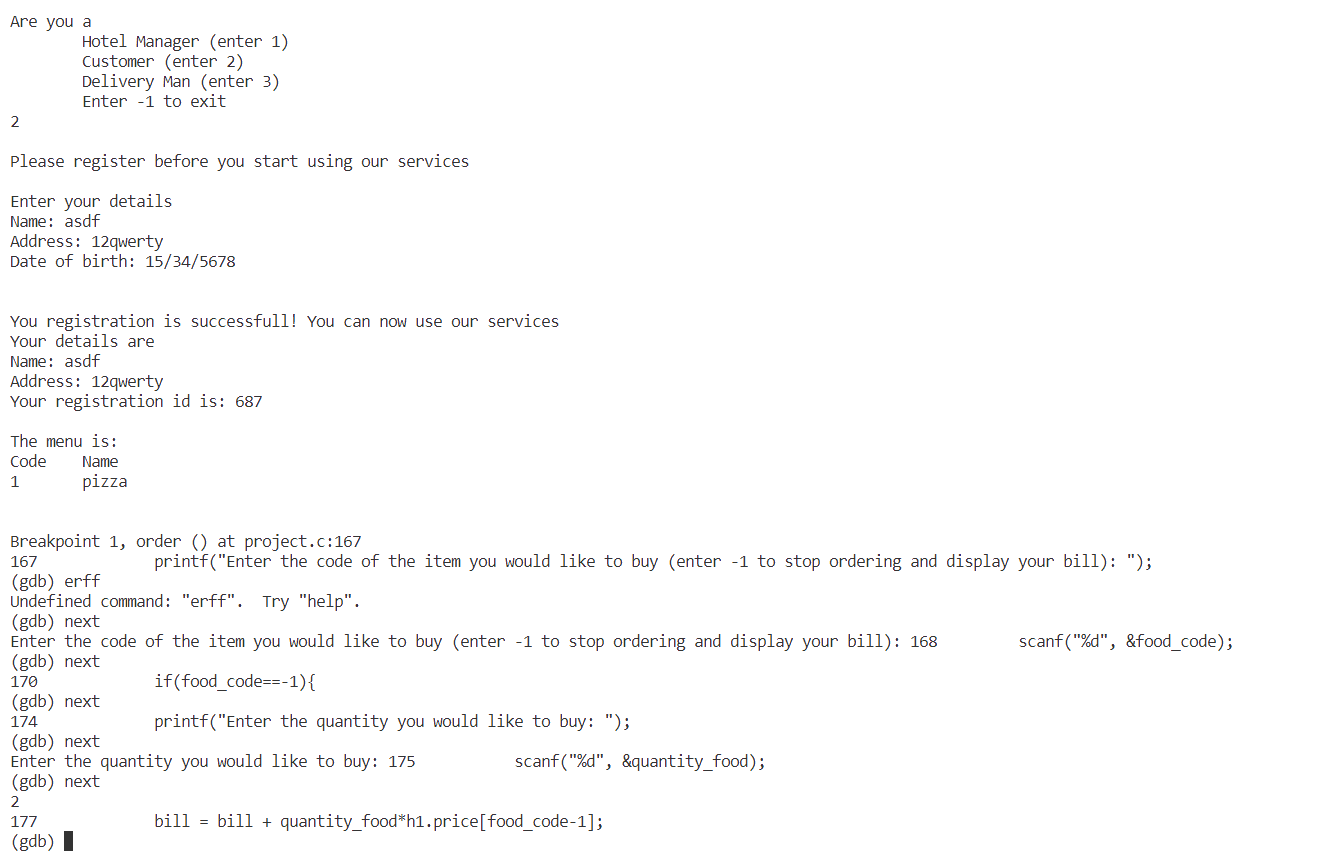
\includegraphics{gdb_2.png}\\

%code with comments
\section{Project Source Code}
\begin{lstlisting}[style=chstyle]
/*
 *Mini Project
 *Food Management System
 */

#include<stdio.h>
#include<stdlib.h>
#include<string.h>
#include<time.h>

struct customer
{
    char name[50];
    char address[50];
    char dob[10];
    int  id;
}c1;

struct hotel
{
    char name[100];
    int registeration_id;
    int password;
    char food[5][20];
    int price[5];
    int count_food;
}h1;

struct delivery
{
    char name[50];
    char vehicle_name[20];
    int vehicle_number;
}d1;

struct management
{
    int delivered_on_time;
    int packaged_properly;
    int complete_order_recieved;
    int bill_recieved;
}m1;

/*
 * This function generates random numbers within a limit using long 
 int as a parameter for the the upper limit. 
 */
int random_number_generator(long int limit){
    
    int temporary = (rand()%(limit+1));
    return temporary;
}


/*
 * This function is used to produce a delay of output during runtime 
 of the program.
 * The amount of time the function needs to delay is taken as a 
 parameter in the function.
 */
void delay(int number_of_seconds)
{

    // seconds are converted into milli seconds because clock 
    measures time in milli seconds
    int milli_seconds = 1000 * number_of_seconds;   
 
    clock_t start_time = clock();

    // empty loop until corresponding time is elapsed
    while (clock() < start_time + milli_seconds){} 
}


/*
 * This function lets the hotel register itself and start using 
 other services
 */
void hotel_login(){
    
    printf("\nEnter your hotel details\n");
    printf("Name: ");
    // getchar is used to empty the input stream containing \n from 
    previous integer input.
    getchar(); 
    // fgets is used to take input of the string using standard 
    input                 
    fgets(h1.name,100,stdin);   

    printf("Password(only in numerical digits): ");
    scanf("%d", &h1.password);
    // this loop is used to confirm the entered password
    while(1){
        int temp;
        printf("Confirm Password: ");
        scanf("%d", &temp);
        if (temp==h1.password)
        {
            break;
        }
    
    }

    // assigning ID to hotel using random number generator.
    h1.registeration_id = random_number_generator(999999999);
    
}

/*
 * This function displays the entered information by user
 */
void display_hotel(){

    printf("\nYou have successfully registered your hotel.\n");
    printf("\t%s", h1.name);
    printf("Here is your registration ID: %d\n", h1.registeration_id);

}


/*
 * This function helps the hotel to create thier menu and list the 
 prices of food.
 */
void hotel_food(){

    printf("\nEnter the food items and its rate you would be serving 
    (Enter X to stop entering itmes):\n");
    int i=0;

    // This loop is used to input the food and its price for the 
    menu
    while(i<5){
        char current_food[20];
        printf("Food: ");
        // getchar is used to empty the input stream containing \n 
        from previous integer input.
        getchar();
        fgets(current_food, 20, stdin);

        if(current_food[0]=='X'){
            break;
        }
        else{
            strcpy(h1.food[i], current_food);

            printf("Price: ");
            scanf("%d", &h1.price[i]);
            i++;
        }

    }
    h1.count_food = i;
    printf("\n");

}


/*
 * This function is used to display the menu to customer while he is 
 ordering food
 */
void display_menu(){

    printf("\nThe menu is:\n");
    printf("Code\tName\n");
    for(int index=0; index<h1.count_food; index++){
        printf("%d\t%s\n", index+1, h1.food[index]);
    }


}


/*
 * This function lets the customer register and use the services.
 */
void customer_login(){
    
    printf("\nEnter your details\n");
    printf("Name: ");
    getchar();
    fgets(c1.name,50,stdin);

    printf("Address: ");
    fgets(c1.address, 50, stdin);

    printf("Date of birth: ");
    fgets(c1.dob, 10, stdin);

    c1.id = random_number_generator(4444);
    printf("\n");

}

/*
 * This function displays the information entered by the customer.
 */
void display_customer(){

    printf("\nYou registration is successfull! You can now use our 
    services\n");
    printf("Your details are\n");
    printf("Name: %s", c1.name);
    printf("Address: %s", c1.address);
    printf("Your registration id is: %d\n", c1.id);

}

/*
 * This function lets the user order food
 */
void order(){

    display_menu();

    // the bill variable starts with zero and increases as the 
    customer orders
    int bill = 0;

    // loop to take the order from customer
    while(1){

        int food_code, quantity_food;
        printf("Enter the code of the item you would like to buy 
        (enter -1 to stop ordering and display your bill): ");
        // getchar is used to empty the input stream containing \n 
        from previous integer input.
        getchar();
        scanf("%d", &food_code);

        if(food_code==-1){
            break;
        }

        printf("Enter the quantity you would like to buy: ");
        scanf("%d", &quantity_food);

        bill = bill + quantity_food*h1.price[food_code-1];

    }

    printf("\nYour bill is %d rupees.\n", bill);


}


/*
 * This function lets the delivery man register.
 */
void delivery_man_login(){

    printf("\nEnter your information\n");
    printf("Name: ");
    // getchar is used to empty the input stream containing \n from 
    previous integer input.
    getchar();
    fgets(d1.name, 50, stdin);
    printf("Vehicle name: ");
    fgets(d1.vehicle_name, 20, stdin);
    printf("Vehicle number: ");
    scanf("%d", &d1.vehicle_number);

}


/*
 * This function displays the delivery information to the customer 
 */
void display_delivery_info(){

    // delay is used to show that the order is being prepared
    delay(4);
    printf("\n\nYour order is on its way\n");
    printf("Delivery Man information is \n");
    printf("Name: %s", d1.name);
    printf("Vehicle name: %s", d1.vehicle_name);
    printf("Vehicle mnumber: %d", d1.vehicle_number);
}


/*
 * this function asks the user for feedback once the order is 
 complete.
 */
void ask_feedback(){

    // delay is being used to show that the order is on its way
    delay(6);
    printf("\n\nYour order is delivered\n");
    printf("\nPlease provide your feedback (enter 1 for satisfied 
    and 0 for not satisfied): \n");
    printf("1. Did you recieved your order on time: ");
    scanf("%d", &m1.delivered_on_time);
    printf("2. Did you recieved your order packaged properly: ");
    scanf("%d", &m1.packaged_properly);
    printf("3. Was the order you recived correct and complte: ");
    scanf("%d", &m1.complete_order_recieved);
    printf("4. Did you recieved bill with your order: ");
    scanf("%d", &m1.bill_recieved);

    printf("\nThank you for providing feedback! Our management team 
    will positively work to improve our services based on your 
    feedback.\n");
}



int main(){


    printf("\n\nWelcome to ABC company\n\n");
    
    // the loop that controls the flow of whole program
    while(1){

        printf("\nAre you a\n\tHotel Manager (enter 1)\n\tCustomer 
        (enter 2)\n\tDelivery Man (enter 3)\n\tEnter -1 to exit\n");
        int field_selector;
        scanf("%d", &field_selector);

        if(field_selector==1){

            printf("\nPlease register before you start using our 
            services\n");

        
            hotel_login();
            display_hotel();
            hotel_food();

        }
        else if(field_selector==2){

            printf("\nPlease register before you start using our 
            services\n");

            customer_login();
            display_customer();
            order();
            printf("Your order will be delivered soon...");
            display_delivery_info();
            ask_feedback();

        }
        else if(field_selector==3){

            delivery_man_login();

        }
        else if(field_selector==-1){
            printf("Thank you for using our services.");
            break;
        }

    }
    

    return 0;
}

\end{lstlisting}

%code output
\section{Code Output}
The output of the program is as follows:\\
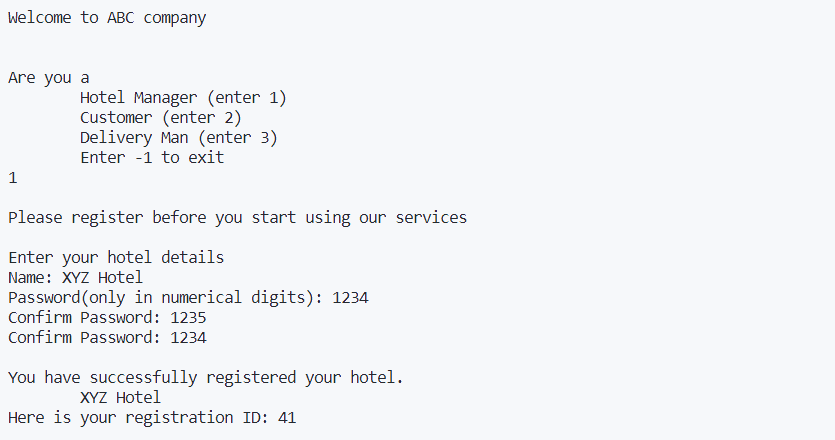
\includegraphics{out_1.png}\\
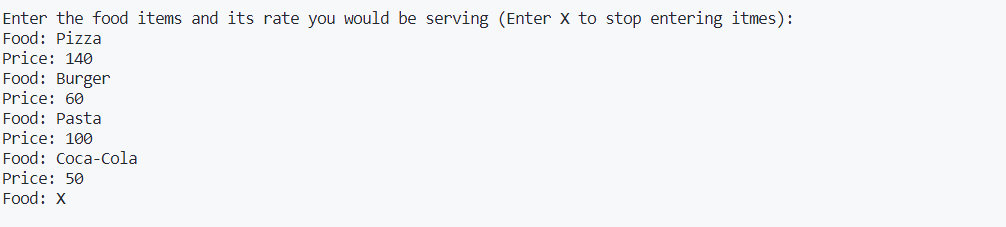
\includegraphics{out_2.png}\\
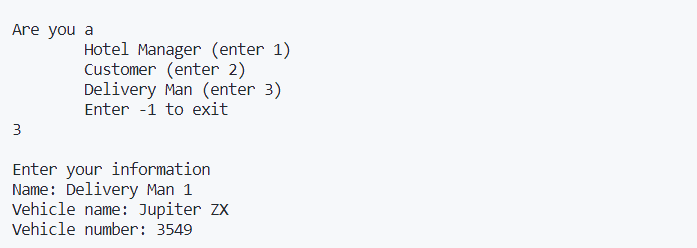
\includegraphics{out_3.png}\\
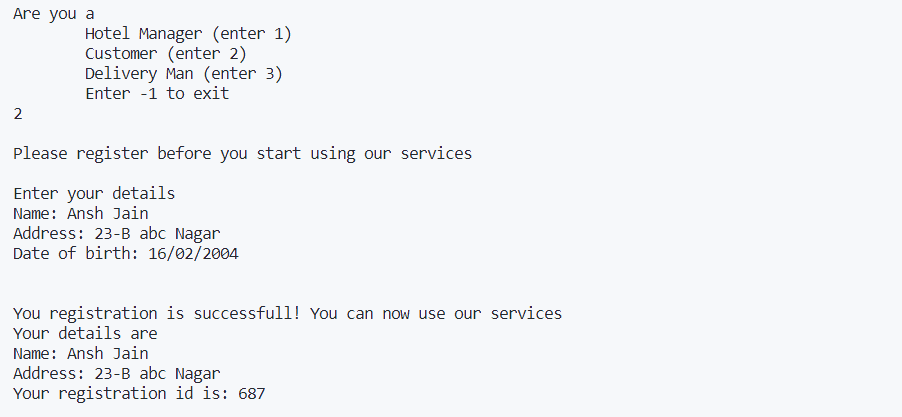
\includegraphics{out_4.png}\\
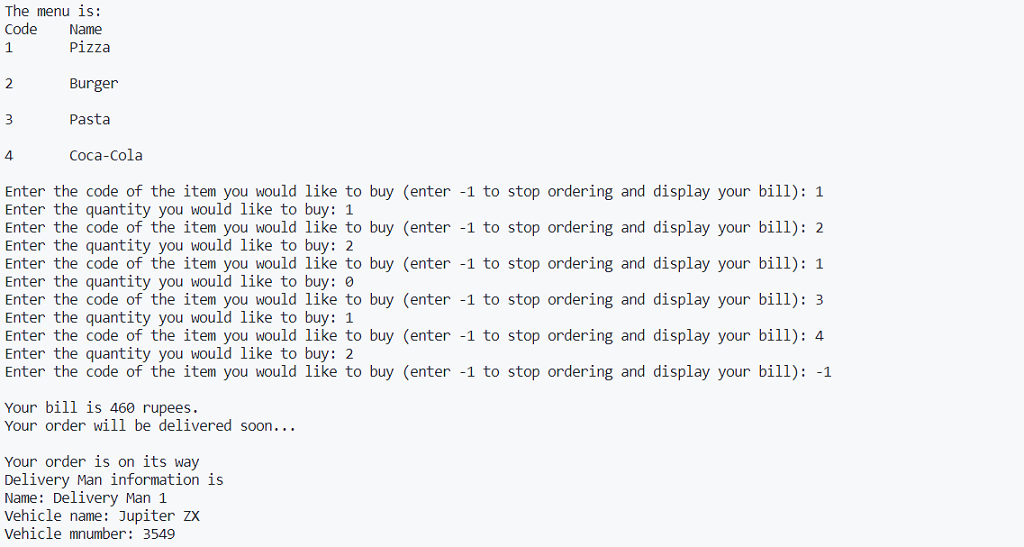
\includegraphics{out_5.png}\\
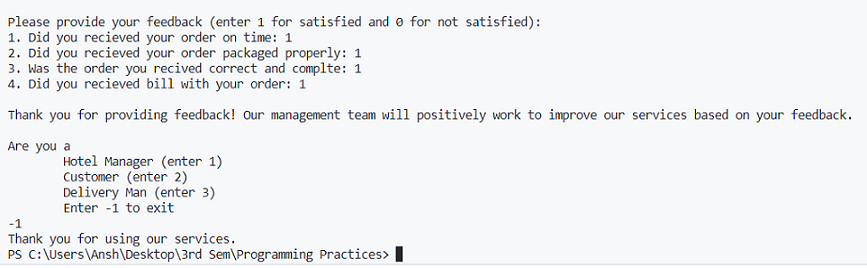
\includegraphics{out_6.png}\\

\end{document}